A Tabela \ref{tab:tempos_shell} apresenta os tempos de execução, em segundos, obtidos para o Shell Sort nos seis tamanhos de instância exigidos pelo trabalho, para cada um dos três tipos de entrada testados.

\begin{table}[htbp]
    \centering
    \begin{tabular}{|l|r|r|r|r|r|r|}
        \hline
         & 10 & 100 & 1.000 & 10.000 & 100.000 & 1.000.000 \\
        \hline
        Crescente & 0,000001 & 0,000001 & 0,000012 & 0,000081 & 0,001082 & 0,017349 \\
        \hline
        Decrescente & 0,000001 & 0,000002 & 0,000012 & 0,000134 & 0,001697 & 0,023871 \\
        \hline
        Random & 0,000001 & 0,000003 & 0,000066 & 0,000821 & 0,011081 & 0,169964 \\
        \hline
    \end{tabular}
    \caption{Tempo de execução (em segundos) do Shell Sort por tamanho e tipo de instância}
    \label{tab:tempos_shell}
\end{table}

O Gráfico \ref{fig:grafico_shell} apresenta esses mesmos dados em escala linear. Diferentemente dos três algoritmos anteriores, mesmo a entrada decrescente permanece com tempo de execução muito baixo -- como discutido na análise de complexidade, uma entrada totalmente decrescente não é o pior caso teórico da sequência de gaps utilizada.

\begin{figure}[htbp]
    \centering
    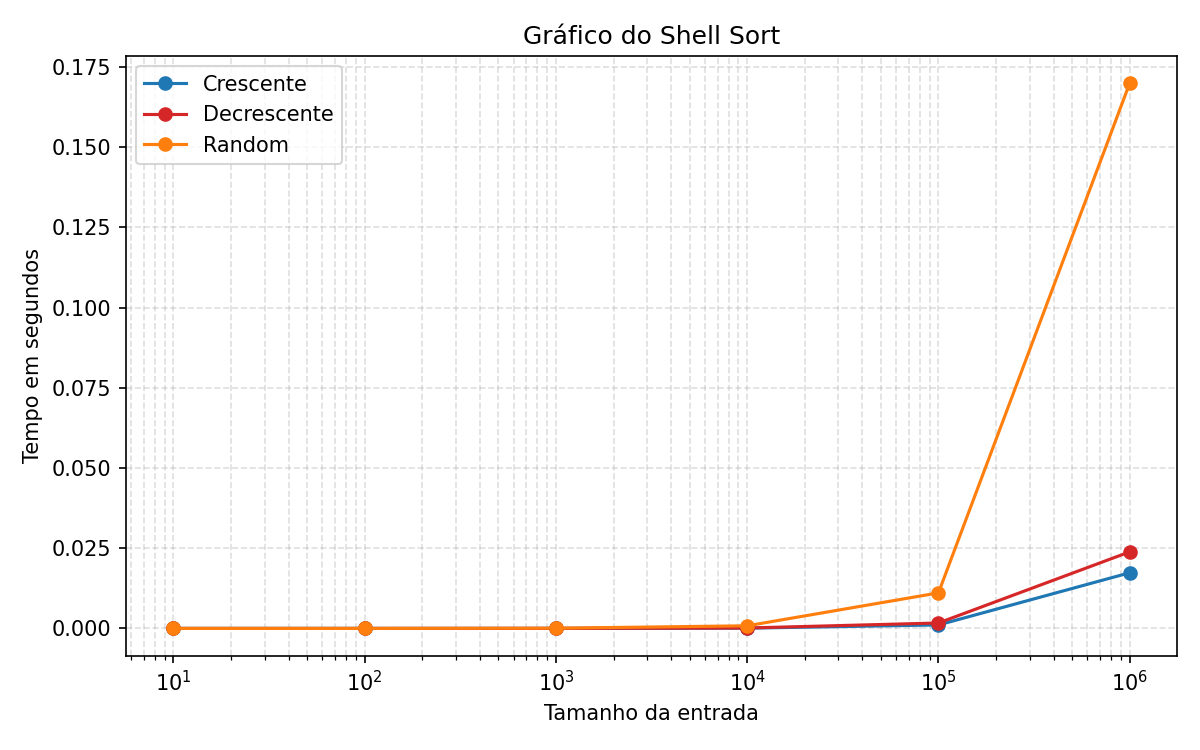
\includegraphics[width=14cm]{Imagens/Shell Sort/grafico.png}
    \caption{Gráfico de tempo por tamanho do algoritmo Shell Sort (escala linear)}
    \label{fig:grafico_shell}
\end{figure}

O Gráfico \ref{fig:grafico_shell_log} em escala logarítmica evidencia que mesmo a entrada randômica, a mais lenta das três para este algoritmo, é ordens de grandeza mais rápida do que qualquer um dos três algoritmos anteriores ($O(n^2)$) para o mesmo tamanho de instância -- a principal conclusão prática deste capítulo, retomada na Tabela de Comparação e no Gráfico Geral ao final deste trabalho.

\begin{figure}[htbp]
    \centering
    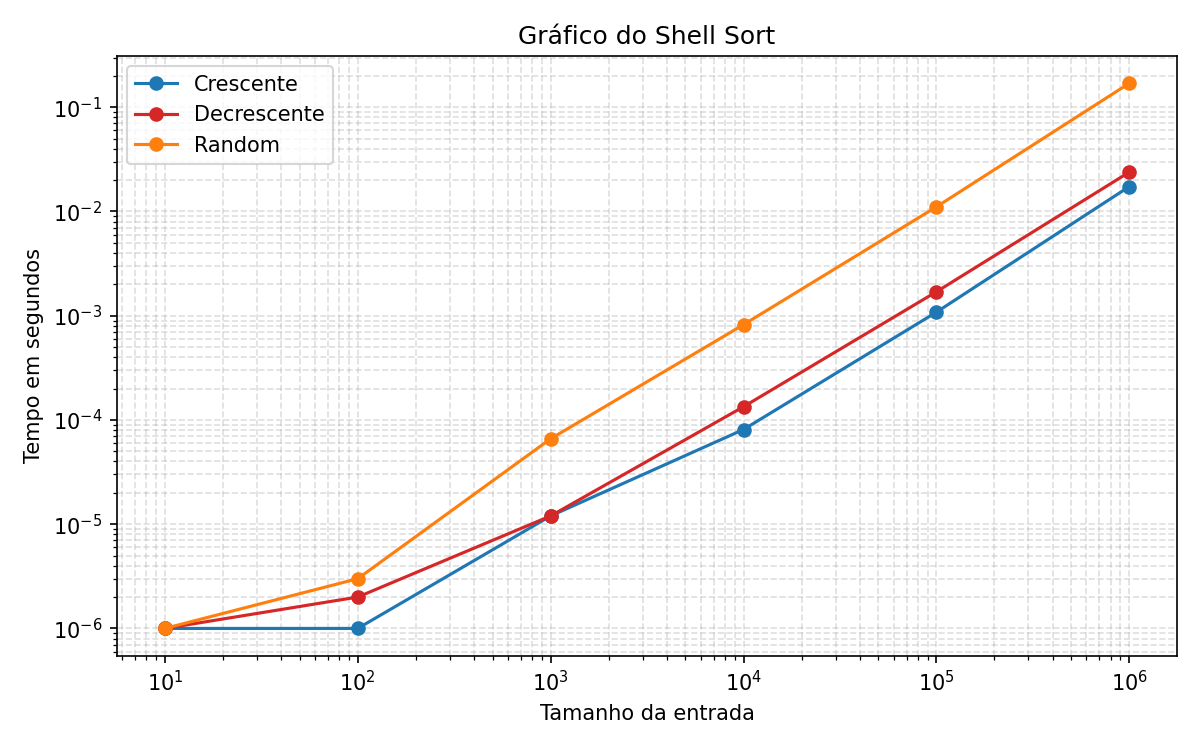
\includegraphics[width=14cm]{Imagens/Shell Sort/grafico_log.png}
    \caption{Gráfico de tempo por tamanho do algoritmo Shell Sort (escala logarítmica)}
    \label{fig:grafico_shell_log}
\end{figure}
